\documentclass{article}

\usepackage[english]{babel}
\usepackage[a4paper,top=2cm,bottom=2cm,left=3cm,right=3cm,marginparwidth=1.75cm]{geometry}

% Useful packages
\usepackage[backend=biber, sorting=nyt, style=authoryear-ibid]{biblatex}
\usepackage[outputdir=pdf]{minted}
\usepackage{graphicx}
\graphicspath{ {figures/} }
\usepackage[colorlinks=true, allcolors=blue]{hyperref}
\usepackage{parskip}
\usepackage{setspace}
\doublespacing
\usepackage{multicol}
\usepackage{multirow}
\usepackage{fontspec}
\usepackage{fontawesome5}
\usepackage{amsmath}
\usepackage{csquotes}

\newcommand{\outlinecite}[1]{\citetitle{#1} \textcite{#1}}
%----------------------------------------------------------------------------------------
%
% Title Page: clear and concise
% e.g. technical report title and module code and title, plus your name and student ID number
%
% Abstract Page
%
% Contents Page {shows structure of report - section numbers, heading andpages}
%
% Introduction {very brief description of
%   aims (general) and
%   objectives (what is done to achieve the aims to put report within context/sets the scene for thereader (e.g. where does this development fit within the field);
%               what are theproblems/issues of the subject area}
%
% Body of report {main part of the report; could be divided in several sectionspending the research/discussions you undertake}
%
% Evaluation {evaluate the results; can be a subsection of the Body of report}
%
% Conclusions {condensed version of body; briefly gives key findings andfuture works}
%
% References (Bibliography) {demonstration of your referencing skills}
%
% Appendices {optional, if there is any}
%
%----------------------------------------------------------------------------------------

\addbibresource{references.bib}

\title{Can Mockingjay Evade your CISO: A Review of Current Process Injection Attacks}
\author{Stuart Kingham}

\begin{document}

\maketitle

\begin{abstract}
  CISOs and boards are not commuicating well with divergent views on the risk of cyber-attacks.
  CISOs should regularly be asking their information security teams to perform risk assessments and mitigation reports that can be used to
  communicate to senior executives and boards on the specific threats to an organisation. 
  In this report we ask if modern End-point Detection Systems (EDR) can provide blanket protection from attacks and what a CISO should be asking from
  their vendors and how attacks can be mitigated.  We review process injection attacks and perform a deep dive review of a modern Windows attack.  We
  ask how well EDRs are able to thwart attacks and highlight the risks of an attack evading an Endpoint Detection System.
\end{abstract}

\newpage
\tableofcontents
\pagenumbering{roman}
\pagenumbering{arabic}

\newpage
\section{Introduction}

% Establish the teritory, the importance and reviewing previous work. how does this assignment relate to cyber-security

\outlinecite{Milica:2023}

\outlinecite{Hiscox:2022}


\subsection{CISO Challenges in Cybersecurity Oversight by Boards}

most directors (65\%) still believe their organizations are at risk of a material cyberattack within the next 12 months, and almost half believe they are unprepared to cope with a targeted attack;  48\% of CISOs share that view. A quarter of boardrooms not viewing cybersecurity as a priority.

\begin{enumerate}
\item Disconnect Between Boards and CISOs: Communication gaps and misalignment impeding progress in cybersecurity.
\item Interactions: To forge strategic partnerships with CISOs, director-CISO engagement between board meetings would enable directors to ask better questions and understand the answers they receive.
\end{enumerate}

Organisations are clearly spending more on cyber-security.  Financial damage is going up. But the HBR report highlights a focus on prevention rather than resiliency.

\begin{figure}[!ht] % Single column figure
  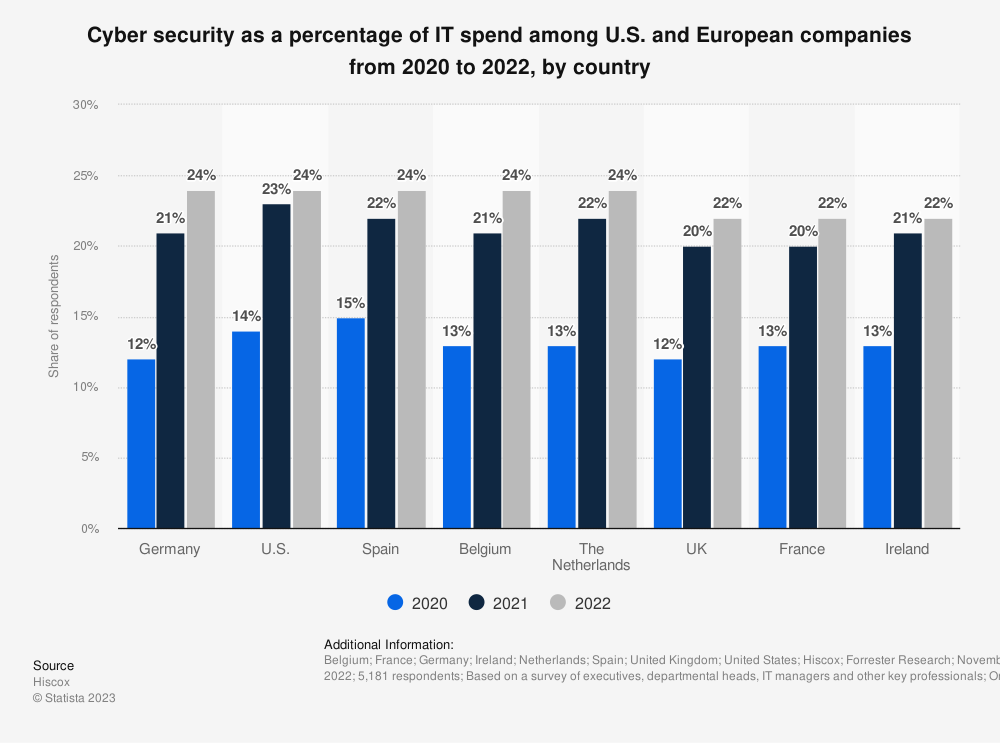
\includegraphics[width=0.95\textwidth]{statistic_id1245356_share-of-it-spend-on-cyber-security-in-the-us-and-europe-2020-2022-by-country.png}\hfill
  \caption{Spending on Cyber Security  \autocite{Hiscox:2022}  Source: Statistica Inc.}
  \label{fig:cybersecurity-spending}
\end{figure}

\begin{figure}[!ht] % Single column figure
  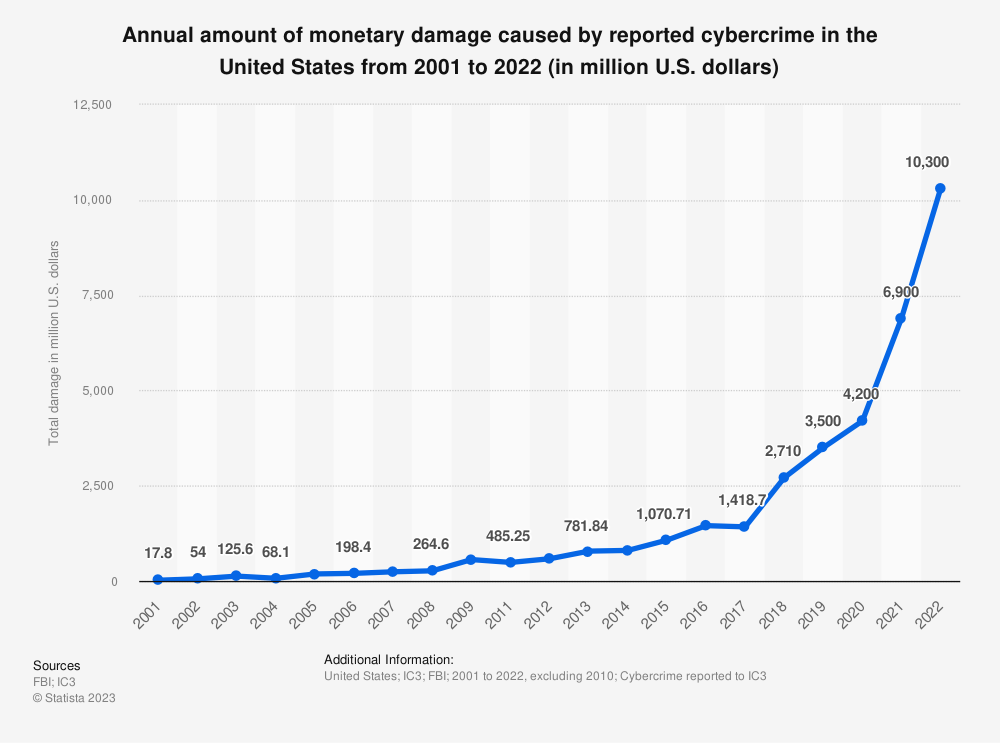
\includegraphics[width=0.95\textwidth]{statistic_id267132_annual-amount-of-financial-damage-caused-by-reported-cybercrime-in-us-2001-2022.png}\hfill
  \caption{Financial Damage caused by Cybercrime in the USA year-on-year \autocite{FBI:2023} Source: Statistica Inc.}
  \label{fig:cybercrime-cost}
\end{figure}

\pagebreak

% Identify a niche, indicating a gap in in knowledge

\subsection{Resilience vs Projection}

\textbf{Importance of addressing issues in cybersecurity oversight by boards}.

\begin{itemize}
\item The necessity of making cybersecurity a continuous priority with ongoing commitment.
\item Focus on Protection Over Resilience:  Boards prioritizing cyber protection despite a high perceived risk.
\item Organizational Risk: Advocacy for a shift towards organizational resilience.
\end{itemize}


\outlinecite{CISA:2023a}:  hijacking legitimate user sessions to generate and execute DLL code in a power shell session

\outlinecite{CVE-2023-3519}: Citrix Netscaler Gateway products vulnerability to launch an unathenitcated remote code expoilt

\outlinecite{CVE-2023-3467}: as well as a privilege escalation attack.

Not email phishind, these are examples of novel attack vectors that  are completely different to the normal social engineering attacks that corporate users are regularly trained to look for and avoid.  While protecing against a users of  email systems on clicking on a nefarious URL link, or opening a spreadsheet, there's rich buffet of choices, new and old, for an attacker to pick from when target targeting a corporation's assets.
as ongoing cybersecurity education about 

\outlinecite{CISA:2023}: Resilience not protection; playbooks ; understanding groups such as ransomware gangs and their techniques.

Relying on EDR systems as a principle defence against a myriad of attacks alieviates many problems.  But it does not alievate the communication gap between company boards


\subsection{Introducing Mockingjay: Importance of understanding process injection techniques.}

It only takes a a few minutes for a new exploit to be found to get access to a companies computing assets.  Citrix have recently reported multiple
vulnerabilies for their Netscaler Gateway products.  Malware identified belonging to the group \textbf{LockBit} have identified hijacking legitimate user sessions to generate and execute DLL code in a power shell session \autocite{CISA:2023a}.  They could as easily used another vulnerability to launch an unatheni \ldots

     \begin{itemize}
\item Cybersecurity as a Technical Topic:
        \item Boards viewing cybersecurity primarily as a technical issue.
        \item Need for a shift from technical to management challenges in discussions.
     \end{itemize}
 

\outlinecite{Peixoto:2023}: a new process injection technique.

\outlinecite{Wang:2022}: in relation to the protections offered by EDR and XDR technologies, and specifically with behaviours that could be used to detect API attacks.

% Occupy the niche; purpose of new research, listing questions, the value of the work and the structure of the writing
\subsection{Purpose of the report: proposing a strategic enhancement for CISOs.}

Board level discusions for cybersecurity oversight:
\begin{itemize}
\item what are the risks to the organisation from cybersecurity incidents
\item what plans are there to manager those risks
\end{itemize}

Boards need to show cbersecurity is a priorty: exemplary heros who has increased resilience of the company.

This paper is a model for the types of analysis that a CISO should be requesting from their information security teams.


\pagebreak
%Section 2
\section{Process Injection Techniques as Malware Attacks on Windows}

\outlinecite{Barabosch:2014}

\begin{figure}[h]
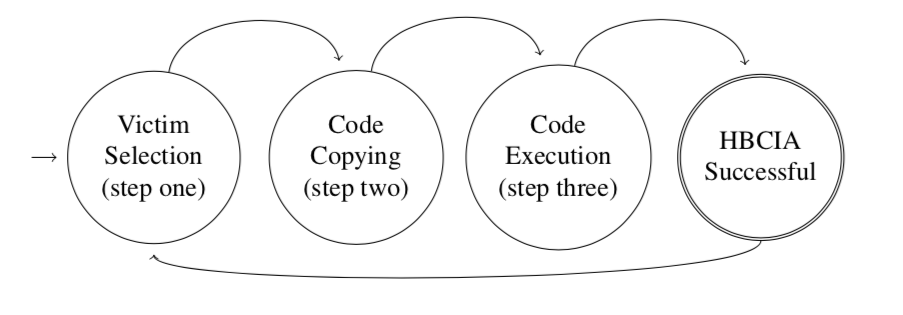
\includegraphics[scale=0.4]{hbcia_3step_algo.png}
\caption{HBCIA Attack Steps \autocite{Barabosch:2014}}
\end{figure}

\outlinecite{Ghizzoni:2004}

\outlinecite{Jang:2007}

\subsection{Code Injection Methods}

\outlinecite{Mitre:2017}

\subsection{Notable malware incidents on Windows platforms}

\subsection{Definition and classification of malware; Overview of process injection}

\subsection{Common vectors for malware distribution and use by Common process injection techniques}

\subsection{Use cases for process injection in malware}

\subsubsection{Evading detection}

\subsubsection{Privilege escalation}

\subsubsection{Payload delivery and execution}

\subsubsection{Deploying Payload into Windows Memory Space}

\outlinecite{Zhan:2018}

\href{https://www.riskinsight-wavestone.com/en/2023/10/process-injection-using-ntsetinformationprocess/}{PI using NTSetInformationProcess}

\href{https://github.com/elddy/Windows-NTAPI-Injector}{NTAPI injector} 

\href{https://gist.github.com/WKL-Sec/96e17188e4c159c2cdf7ff2c111130cc#file-local-c}{Injector examples in C}

\href{https://www.unknowncheats.me/forum/anti-cheat-bypass/286274-internal-detection-vectors-bypass.html}{internal detection vectors bypass}

\href{https://medium.com/@s12deff/process-injection-with-random-rwx-memory-spaces-3e3651149527}{PI with random RWX memory spaces}


\textbf{\citetitle{Dequeker:2023}}: \autocite{Dequeker:2023}

\textbf{Keywords}: NtSetInformationProcess, Nirvana debugging, Process injection, Code injection, Execution hijacking, Unhooking, Bypass.

The NtSetInformationProcess function can be used to register a callback that executes after every system call made by a process. This Nirvana callback can be set on a remote process if the SE\_DEBUG privilege is enabled.

The key advantage of this technique is bypassing hooks and behavioral monitoring of common process injection APIs. The disadvantage is it requires elevation and debug privileges to target a remote process.
By writing shellcode into the target process that registers a Nirvana callback, and writing a payload (in this case Cobalt Strike) to another memory location in the target process, the shellcode callback can execute the payload after the next system call.

So this allows arbitrary code execution in the context of a remote process without using the typical functions monitored by security products like VirtualAllocEx, WriteProcessMemory, and CreateRemoteThread.

This technique attempts to use a lesser-known API function in an unconventional way to bypass hooks, behavior monitoring, and other detection that focuses on common injection techniques. The kernel-mode execution flow also helps evade user-mode security mechanisms.

\begin{figure}[ht]
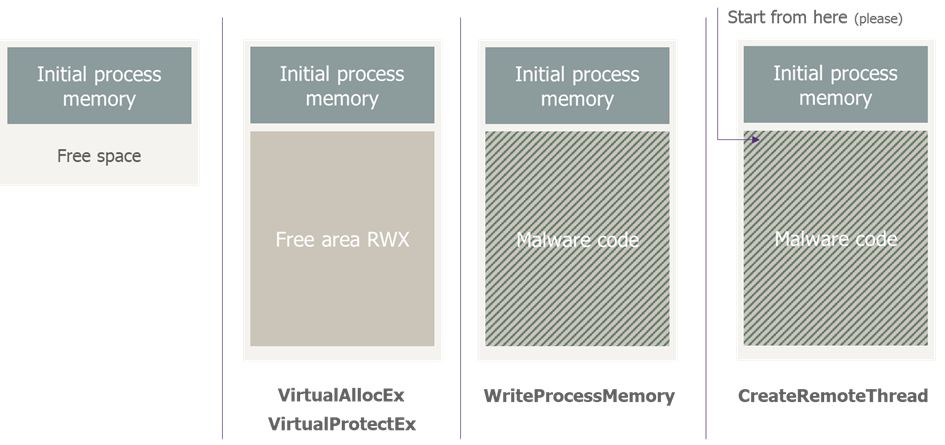
\includegraphics[scale=0.9]{dequeker_standard_process_injection_pattern.png}
\caption{Standard process Injection pattern \autocite{Dequeker:2023}}
\end{figure}
 

\subsection{Detection and Mitigation}

\subsubsection{Current strategies for detecting process injection}

\subsubsection{Anti-malware tools and techniques}

\subsubsection{Best practices for preventing and mitigating process injection attacks}

\section{EDRs Response to an Evolving Threat Landscape}

\outlinecite{Hayes:2023}

\subsection{Emerging trends in malware attacks on Windows}

\subsection{Advancements in process injection techniques}

\subsection{Future predictions for the evolution of these threats}



%\section{Proess Injection Attack and EDR Repsonse Primer}
\section{Case Study: Introducing MockingJay; New Process Injection Attacks}

\textbf{Key problems and issues}
\begin{itemize}
\item Security Joes, an Incident Response company that specializes in IR, MDR \& Red Teaming, has created a novel process injection
  exploit that bypasses allocation and permission API hooks used by EDRs.  By using existing RWX code sections and without starting threads...self injection and remote injection.
\item Recent Citrix Netscaler CVE was issued: software vulnerability found in Citrix NetScaler ADC and NetScaler Gateway appliances with exploitation activity identified as early as August 2023. This vulnerability provides threat actors, including LockBit 3.0 ransomware affiliates, the capability to bypass MFA [T1556.006] and hijack legitimate user session,
\item It is realistic to assume that an attack cannot be prevented with 100\% certainly.  WIth this assumption we nee
\end{itemize}

\textbf{Thesis statement and outcome}
\begin{itemize}
\item Review Mitigants for attacks that can be anticipated from the problems identified.
\item Engage with our EDR/XDR vendor to request a response to this attack vector and test for 
\item Review our run books for
  \item Bolster our Cybersecurity Framework (CSF) functions, as defined by NIST.
\end{itemize}



It only takes a a few minutes for a new exploit to be found to get access to a companies computing assets.  Citrix have recently reported multiple
vulnerabilies for their Netscaler Gateway products.  Malware identified belonging to the group \textbf{LockBit} have identified hijacking legitimate user sessions to generate and execute DLL code in a power shell session \autocite{CISA:2023a}.  They could as easily used another vulnerability to launch an unathenitcated remote code expoilt, \autocite{CVE-2023-3519}, as well as a privilege escalation attack \autocite{CVE-2023-3467}.  These are examples of novel attack vectors that  are completely different to the normal social engineering attacks that corporate users are regularly trained to look for and avoid.  While protecing against a users of  email systems on clicking on a nefarious URL link, or opening a spreadsheet, there's rich buffet of choices, new and old, for an attacker to pick from when target targeting a corporation's assets.

For organisations with assets that threat actors want to attack, it's necessary to at a minimum keep abreast of both reported Common Vulnerability and Exposures (CVE)
security flaws of their systems, published by NIST and MITRE, and reviewing advisories such as those issued by the Cybersecurity and Infrastructure Security Agency (CISA)
as ongoing cybersecurity education about groups such as ransomware gangs and their techniques \autocite{CISA:2023}.
% \href{https://www.cshub.com/attacks/articles/five-active-ransomware-gangs-and-their-tactics-part-one}{tactics} are a vital part of an organisation's cyber-security education and defence.


% \subsection{Real-world examples of malware employing process injection on Windows}
\subsection{Context: Detailed analysis of new process injection attacks.}


\href{https://www.securityjoes.com/post/process-mockingjay-echoing-rwx-in-userland-to-achieve-code-execution}{Mockingjay echoing in userland to achieve code execution}

\href{https://www.linkedin.com/posts/john-stigerwalt-90a9b4110_mockingjay-memory-allocation-primitive-activity-7083050050158743552-Hgyw}{mockingjay memory allocation primative}

\href{https://whiteknightlabs.com/2023/07/06/mockingjay-memory-allocation-primitive/}{white knights mocking jay}

\textbf{\textcite{Inam:2023}: Provenance-based system auditing and how it could improve EDR malware detection}


\subsection{Alternatives: how these attacks could potentially evade EDR}


% \subsection{Analysis of the impact and consequences of these incidents}
\subsection{Proposed Solution: assessing and improving the organization's cybersecurity measures.}
\textbf{Resilience: Detect and Respond phases of NIST CSF Functions}

\href{https://www.cert.govt.nz/it-specialists/guides/how-ransomware-happens-and-how-to-stop-it/}{how-ransomware-happens-and-how-to-stop-it}

\begin{figure}[ht]
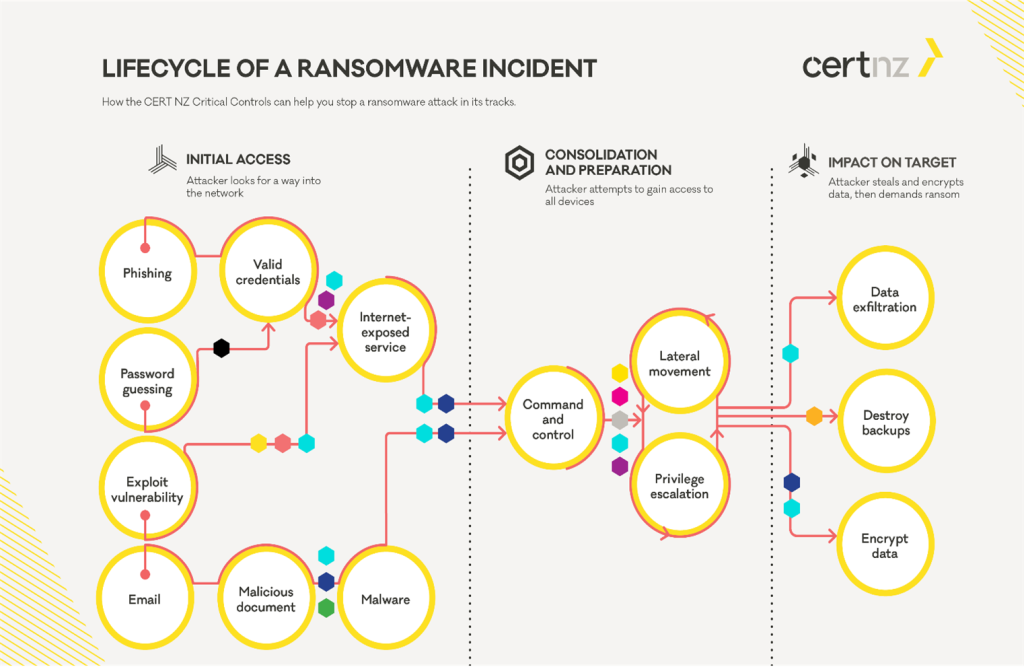
\includegraphics[scale=0.4]{certnz_aa23-165a.png}
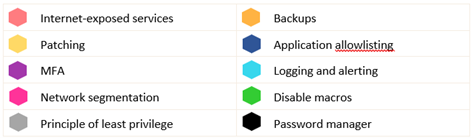
\includegraphics[scale=0.6]{certnz_aa23-165b.png}
\caption{Ransomeware Layered Mitigations \autocite{Certnz:2021}}
\end{figure}

\subsection{Recommendations}

\begin{itemize}
\item Identify: review EDR/MDF/XDR solution to ensure we are mitigating known vulnerabilities
\item Protect: review XDR solutions are monitoring log files to detect encryption; use technique to find vulnerable exes and block them (eg. visual studio ssh exfiltration block known malicios systes
\item Detect: XDR are able to detect loading of NTDLL.dll from disk
\item Respond: Ensure that our organisation is able to report to all relevant authorities  and abide to our legal responsibilities for disclosuress
\item Recover: review perform disaster recover tests to restore systems from backups and that backups are immutable 
\item Continued review of new research and reported attacks
\end{itemize}


\pagebreak
\section{So How Hard is this Anyway?  Attack!}

\subsection{Inoculation: Generating artifacts}



\pagebreak
\section{Conclusion}

\pagebreak
\printbibliography

\end{document}

%%% Local Variables:
%%% mode: latex
%%% TeX-master: t
%%% End: